% Permission is granted to copy, distribute and/or modify this document
% under the terms of the GNU Free Documentation License, Version 1.3
% or any later version published by the Free Software Foundation;
% with no Invariant Sections, no Front-Cover Texts, and no Back-Cover Texts.
% A copy of the license is included in the section entitled "GNU
% Free Documentation License".
%
% Written (C) 2012 Heiko Strathmann

\section{Two-Sample-Testing with the Maximum Mean Discrepancy}
\label{sec:mmd_into}
In two-sample testing, one tries to find out whether to sets of samples come from different distributions. Given two probability distributions $p,q$ and i.i.d.\ samples $X=\{x_i\}_{i=1}^m\subseteq \mathbb{R}^d\sim p$ and $Y=\{y_i\}_{i=1}^n\subseteq \mathbb{R}^d\sim p$, the two sample test distinguishes the hypothesises
\begin{align*}
H_0: p=q\\
H_A: p\neq q
\end{align*}

In order to solve this problem, it is desirable to have a criterion than takes a positive unique value if $p\neq q$, and zero if and only if $p=q$. The so called \emph{Maximum Mean Discrepancy} (MMD), has this property and allows to distinguish any two probability distributions, if used in a \emph{reproducing kernel Hilbert space} (RKHS). It is the distance of the mean embeddings $\mu_p, \mu_q$ of the distributions $p,q$ in such a RKHS $\mathcal{F}$ -- which can also be expressed in terms of expectation of kernel functions, i.e.
\begin{align}
\label{eqn:mmd_population}
\mmd[\mathcal{F},p,q]&=||\mu_p-\mu_q||_\mathcal{F}^2\\
&=\textbf{E}_{x,x'}\left[ k(x,x')\right]-
  2\textbf{E}_{x,y}\left[ k(x,y)\right]
  +\textbf{E}_{y,y'}\left[ k(y,y')\right]\notag
\end{align}
See \citep[Section 2]{Gretton2012} for details. We here only describe how to
use the MMD for two-sample testing. \shogun{} offers two types of test statistic based on the MMD, one with quadratic costs both in time and space, and on with linear time and constant space costs. Both come in different versions and with different methods how to approximate the null-distribution in order to construct a two-sample test.

\subsection{Quadratic Time MMD Statistic}
\label{sec:mmd_quadratic}
We now describe the quadratic time MMD, as described in \citep[Lemma
6]{Gretton2012}, which is implemented in \shogun{}. All methods in this section are implemented in \shogunclass{CQuadraticTimeMMD}.

An unbiased estimate for expression \ref{eqn:mmd_population} can be obtained by estimating expected values with sample means
\begin{align*}
\mmd_u^2[\mathcal{F},X,Y]=&\frac{1}{m(m-1)}\sum_{i=1}^m\sum_{j\neq i}^mk(x_i,x_j) + \frac{1}{n(n-1)}\sum_{i=1}^n\sum_{j\neq i}^nk(y_i,y_j)\\
&-\frac{2}{mn}\sum_{i=1}^m\sum_{j\neq i}^nk(x_i,y_j)
\end{align*}

A biased estimate would be
\begin{align*}
\mmd_b^2[\mathcal{F},X,Y]=&\frac{1}{m^2}\sum_{i=1}^m\sum_{j=1}^mk(x_i,x_j) + \frac{1}{n^ 2}\sum_{i=1}^n\sum_{j=1}^nk(y_i,y_j)\\
&-\frac{2}{mn}\sum_{i=1}^m\sum_{j\neq i}^nk(x_i,y_j)
\end{align*}

To compute statistic, use \texttt{compute\_statistic}. To decide which statistic to use, use \texttt{set\_statistic\_type} with arguments \texttt{BIASED} or \texttt{UNBIASED} to activate this statistic type. Note that some methods for approximating the null-distribution only work with one of both types. Both statistics' computational costs are quadratic both in time and space. Note that the method returns $m\mmd_b^2[\mathcal{F},X,Y]$ since null distribution approximations work on $m$ times null distribution.

\subsubsection{Bootstrapping}
As for any two-sample test in \shogun{}, bootstrapping can be used to approximate the null-distribution with both types of quadratic MMD statistic. This results in a consistent, but slow test. Note that for each sample, the quadratic time estimate has to be re-computed. The number of samples to take is the only parameter. As a rule of thumb, use at least 250 samples.
See \texttt{bootstrap\_null} in \shogunclass{CTwoDistributionsTestStatistic} and \shogunclass{CKernelTwoSampleTestStatistic}. Strongly consider using pre-computed kernel matrices as described in section \ref{sec:quadratic_mmd_precomputed_kernel}.

\subsubsection{Spectrum Approximation}
Approximates the null-distribution using the Eigen-Spectrum of the kernel matrix of the joint samples. Was described in \citep{Gretton2012b}. This is a fast and consistent test. Effectively, the null-distribution of the biased statistic is sampled, but in a more efficient way than the bootstrapping approach. The converges as

\begin{align}
\label{eqn:quadratic_mmd_spectrum}
m\mmd^2_b \rightarrow \sum_{l=1}^\infty \lambda_l z_l^2
\end{align}
where $z_l\sim \mathcal{N}(0,2)$ are i.i.d. normal samples and $\lambda_l$
Eigenvalues of expression 2 in \citep{Gretton2012b}, which can be empirically
estimated by $\hat\lambda_l=\frac{1}{m}\nu_l$ where $\nu_l$ are the Eigenvalues
of the centred kernel matrix of the joint samples $X$ and $Y$. The distribution
in expression \ref{eqn:quadratic_mmd_spectrum} can be easily sampled. \shogun{}'s implementation has two parameters:
\begin{itemize}
\item Number of samples from null-distribution. The more, the more accurate. As a rule of thumb, use 250.
\item Number of Eigenvalues of the Eigen-decomposition of the kernel matrix to use. The more, the better the results get; however, the Eigen-spectrum of the joint gram matrix usually decreases very fast. See \citep{Gretton2012b} for details.
\end{itemize}
If the kernel matrices are diagonal dominant, this method is likely to fail. For that and more details, see the original paper. Computational costs are much lower than bootstrapping, which is the only consistent alternative. Since Eigenvalues of the gram matrix has to be computed, costs are in $\mathcal{O}(m^3)$.

To get a number of samples, use \texttt{sample\_null\_spectrum}; to use that method for testing, use \texttt{set\_null\_approximation\_method(MMD2\_SPECTRUM)}. Both methods are to be found in \shogunclass{CQuadraticTimeMMD}. Important: This method only works with the biased statistic.
\subsubsection{Gamma Approximation}
Another method for approximating the null-distribution is by matching the first two moments of a gamma-distribution and then use that. This is not consistent, but usually also gives good results while being very fast. However, there are distributions where the method fails; therefore, the type I error should always be monitored. Described in \citep{Gretton2012b}. It uses
\begin{align}
\label{eqn:quadratic_mmd_gamma}
m\mmd_b(Z) \sim \frac{x^{\alpha-1}\exp(-\frac{x}{\beta})}{\beta^\alpha \Gamma(\alpha)}
\end{align}
where
\begin{align*}
\alpha=\frac{(\textbf{E}(\text{MMD}_b(Z)))^2}{\var(\text{MMD}_b(Z))} \qquad \text{and} \qquad
 \beta=\frac{m \var(\text{MMD}_b(Z))}{(\textbf{E}(\text{MMD}_b(Z)))^2}
\end{align*}

Then, any threshold and p-value can be computed using the gamma distribution in expression \ref{eqn:quadratic_mmd_gamma}. Computational costs are in $\mathcal{O}(m^2)$.

To use that method for testing, use \texttt{set\_null\_approximation\_method(MMD2\_GAMMA)}, to be found in \shogunclass{CQuadraticTimeMMD}. Important: This method only works with the biased statistic.


\subsection{Linear Time MMD Statistic}
\label{sec:mmd_linear}
We now describe the linear time MMD, as described in \citep[Section
6]{Gretton2012}, which is implemented in \shogun{}. All methods in this section are implemented in \shogunclass{CLinearTimeMMD}.

An fast, unbiased estimate for expression \ref{eqn:mmd_population} which still uses all available data can be obtained by dividing data into two parts and then compute

\begin{align*}
\mmd_l^2[\mathcal{F},X,Y]=\frac{1}{m_2}\sum_{i=1}^{m_2} k(x_{2i},x_{2i+1})+k(y_{2i},y_{2i+1})-k(x_{2i},y_{2i+1})-
  k(x_{2i+1},y_{2i})
\end{align*}
where $ m_2=\lfloor\frac{m}{2} \rfloor$. This statistic is interesting for large scale tests since its computational costs are linear in the number of samples; and the space costs are constant -- it is therefore very suitable for large amounts of streaming data. To compute statistic, use \texttt{compute\_statistic}.

\subsubsection{Bootstrapping}
As for any two-sample test in \shogun{}, bootstrapping can be used to approximate the null distribution. This results in a consistent, but slow test. The number of samples to take is the only parameter. As a rule of thumb, use at least 250 samples.
See \texttt{bootstrap\_null} in \shogunclass{CTwoSampleTestStatistic}. Note that this method is not really necessary since with the Gaussian approximation, a fast and consistent estimate of the null-distribution is available for the linear time MMD.

\subsubsection{Gaussian Approximation}
Since both the null- and the alternative distribution are Gaussians with equal variance (and different mean), it is possible to approximate the null-distribution by using a linear time estimate for this variance. An unbiased, linear time estimator for
\begin{align*}
\var[\mmd_l^2[\mathcal{F},X,Y]]
\end{align*}
can simply be computed by computing the empirical variance of
\begin{align*}
k(x_{2i},x_{2i+1})+k(y_{2i},y_{2i+1})-k(x_{2i},y_{2i+1})-k(x_{2i+1},y_{2i}) \qquad (1\leq i\leq m_2)
\end{align*}
A normal distribution with this variance and zero mean can then be used as an approximation for the null-distribution. This results in a consistent test and is very fast. The approximation gets accurate from about $m=1000$.

To use that method for testing, use \texttt{set\_null\_approximation\_method(MMD1\_GAUSSIAN)}, to be found in \shogunclass{CLinearTimeMMD}.

\subsection{Precomputed Kernel Matrices for Quadratic Time MMD}
\label{sec:quadratic_mmd_precomputed_kernel}
For all MMD-based two-sample-tests, elements of kernel matrices of sample data have to be used. By default, all computations are done \emph{in-place} when possible, which means that the underlying kernel is evaluated on the fly (There are exceptions, when the matrix has to be stored, for example in order so solve Eigenvalue problems). However, for the quadratic time MMD, this may be inefficient when statistics are computed multiple times -- as in bootstrapping. Therefore, it is possible to initialize \shogunclass{CQuadraticTimeMMD} with a pre-computed \shogunclass{CCusotmKernel}. This kernel may be computed from any other kernel by simply passing the latter to the constructor of \shogunclass{CCusotmKernel}. This should be done whenever the kernel matrix fits into memory; it greatly improves performance. In bootstrapping, the kernel matrix only has to be permuted instead of being re-computed in every iteration. But there is also a (small) advantage for all other methods since \shogun{} computes kernel matrices in multiple threads.

In contrast, \shogunclass{CLinearTimeMMD} should not be used with \shogunclass{CCusotmKernel}s since it does not even need all elements -- so pointless computations would be made. Also, \shogunclass{CLinearTimeMMD} might be changed to work on stream data only in the future.

\subsubsection{Examples}
There are graphical python examples which plot example data, alternative and null-distributions. See figures \ref{fig:statistical_testing-quadratic_time_mmd} and \ref{fig:statistical_testing-linear_time_mmd} for a screenshot for quadratic and linear time MMD respectively.

\begin{figure}\centering
		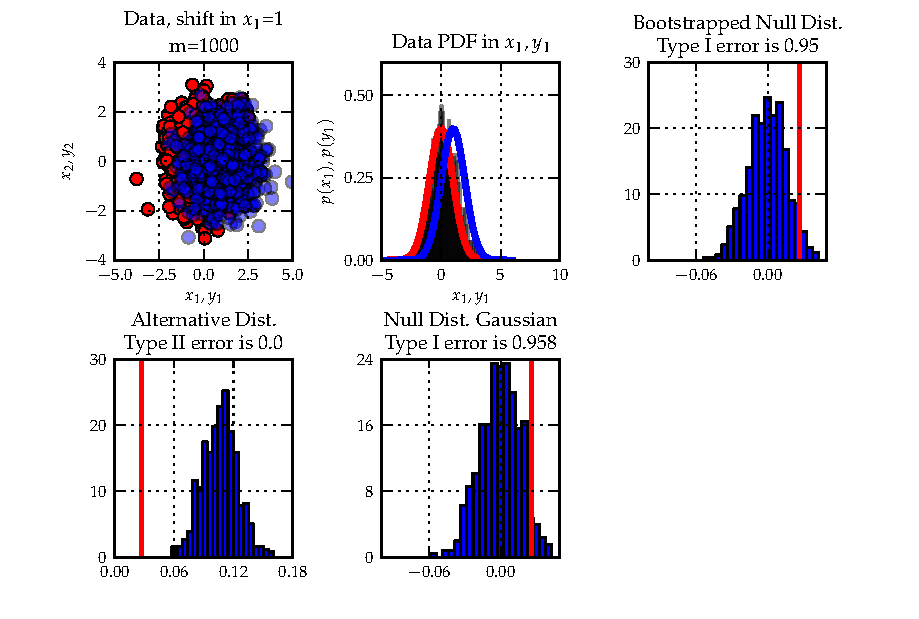
\includegraphics{fig/statistical_testing/linear_time_mmd}
		\caption{Screenshot of graphical python example for linear time MMD.}
		\label{fig:statistical_testing-linear_time_mmd}
\end{figure}

\begin{figure}\centering
		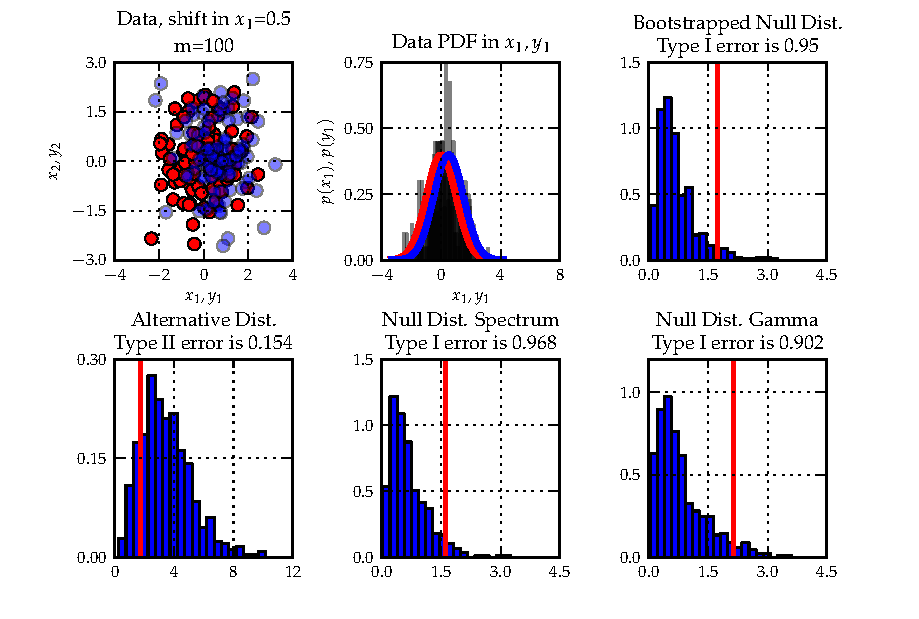
\includegraphics{fig/statistical_testing/quadratic_time_mmd}
		\caption{Screenshot of graphical python example for quadratic time MMD.}
		\label{fig:statistical_testing-quadratic_time_mmd}
\end{figure}